\documentclass[
	a4paper,
	oneside,
	BCOR = 10mm,
	DIV = 12,
	12pt,
	headings = normal,
]{scrartcl}

%%% Length calculations
\usepackage{calc}
%%%

%%% Support for color
\usepackage{xcolor}
\definecolor{lightblue}{HTML}{03A9F4}
\definecolor{red}{HTML}{F44336}
%%%

%%% Including graphics
\usepackage{graphicx}
%%%

%%% Font selection
\usepackage{fontspec}

\setromanfont{STIX Two Text}[
	SmallCapsFeatures = {LetterSpace = 8},
]

\setsansfont{IBM Plex Sans}[
	Scale = MatchUppercase,
]

\setmonofont{IBM Plex Mono}[
	Scale = MatchUppercase,
]
%%%

%%% Math typesetting
\usepackage{amsmath}

\usepackage{unicode-math}
\setmathfont{STIX Two Math}
%%%

%%% List settings
\usepackage{enumitem}
\setlist[enumerate]{
	label*      = {\arabic*.},
	leftmargin  = *,
	labelindent = \parindent,
	topsep      = 1\baselineskip,
	parsep      = 0\baselineskip,
	itemsep     = 1\baselineskip,
}

\setlist[itemize]{
	label*      = {—},
	leftmargin  = *,
	labelindent = \parindent,
	topsep      = 1\baselineskip,
	parsep      = 0\baselineskip,
	itemsep     = 1\baselineskip,
}

\setlist[description]{
	font        = {\rmfamily\upshape\bfseries},
	topsep      = 1\baselineskip,
	parsep      = 0\baselineskip,
	itemsep     = 0\baselineskip,
}

%%%

%%% Structural elements typesetting
\setkomafont{pagenumber}{\rmfamily}
\setkomafont{disposition}{\rmfamily\bfseries}

% Sectioning
\RedeclareSectionCommand[
	beforeskip = -1\baselineskip,
	afterskip  = 1\baselineskip,
	font       = {\normalsize\bfseries\scshape},
]{section}

\RedeclareSectionCommand[
	beforeskip = -1\baselineskip,
	afterskip  = 1\baselineskip,
	font       = {\normalsize\bfseries\itshape},
]{subsection}

\RedeclareSectionCommand[
	beforeskip = -1\baselineskip,
	afterskip  = 1\baselineskip,
	font       = {\normalsize\bfseries},
]{subsubsection}

\RedeclareSectionCommand[
	beforeskip = -1\baselineskip,
	afterskip  = -0.5em,
	font       = {\normalsize\mdseries\scshape\addfontfeatures{Letters = {UppercaseSmallCaps}}},
]{paragraph}
%%%

%%% Typographic enhancements
\usepackage{microtype}
%%%

%%% Language-specific settings
\usepackage{polyglossia}
\setmainlanguage{ukrainian}
\setotherlanguages{english}
%%%

%%% Captions
\usepackage{caption}
\usepackage{subcaption}

%\DeclareCaptionLabelFormat{closing}{#2)}
%\captionsetup[subtable]{labelformat = closing}

%\captionsetup[subfigure]{labelformat = closing}

\captionsetup[table]{
	aboveskip = 0\baselineskip,
	belowskip = 0\baselineskip,
}

\captionsetup[figure]{
	aboveskip = 1\baselineskip,
	belowskip = 0\baselineskip,
}

\captionsetup[subfigure]{
	labelformat = simple,
	labelformat = brace,
}
%%%

%%% Table typesetting
\usepackage{booktabs}
\usepackage{longtable}

\usepackage{multirow}

\usepackage{array}
\newcolumntype{v}[1]{>{\raggedright\arraybackslash\hspace{0pt}}p{#1}}
\newcolumntype{b}[1]{>{\centering\arraybackslash\hspace{0pt}}p{#1}}
\newcolumntype{n}[1]{>{\raggedleft\arraybackslash\hspace{0pt}}p{#1}}
%%%

%%% Drawing with TikZ
% \usepackage{tikz}
% \usepackage{tikzscale}
% \usetikzlibrary{
% 	arrows.meta, % Stealth arrow tips
% 	positioning,
% 	shapes,
% 	trees,
% }

% \tikzset{> = stealth}
%%%

%%% PDF inclusion
\usepackage{pdfpages}
%%%

%%% Links and hyperreferences
\usepackage{hyperref}
\hypersetup{
	bookmarksnumbered = true,
	colorlinks      = false,
	linkbordercolor = red,
	urlbordercolor  = lightblue,
	pdfborderstyle  = {/S/U/W 1.5},
}
%%%

%%% Length adjustments
% Set baselineskip, default is 14.5 pt
\linespread{1.068966} % ~15.5 pt
\setlength{\emergencystretch}{1em}
\setlength{\parindent}{1.5em}
\newlength{\gridunitwidth}
\setlength{\gridunitwidth}{\textwidth / 12}
%%%

%%% Custom commands
\newcommand{\allcaps}[1]{{\addfontfeatures{LetterSpace = 8, Kerning = Off}#1}}
%%%

\begin{document}
	\begin{titlepage}
		\begin{center}
			Міністерство освіти і науки України\\
			Національний авіаційний університет\\
			Навчально-науковий інститут комп'ютерних інформаційних технологій\\
			Кафедра комп'ютеризованих систем управління

			\vspace{\fill}
				Лабораторна робота №1.3\\
				з дисципліни «Інженерія програмного забезпечення»\\
				на тему «Графік робіт проекту і перегляд критичного шляху»\\
				Варіант №3

			\vspace{\fill}

			\begin{flushright}
				Виконав:\\
				студент ННІКІТ\\
				групи СП-325\\
				Клокун В.\,Д.\\
				Перевірила:\\
				Голего Н.\,М.
			\end{flushright}

			Київ 2018
		\end{center}
	\end{titlepage}

	\section{Мета}
		Побудова графіку робіт засобами \textenglish{Microsoft Project}.

	\section{Завдання}
		Побудувати графік виконання робіт із~проектування~\allcaps{ІС} та~визначити критичний шлях.
		
	\section{Хід роботи}
	% \paragraph{Проект та базовий календар}
		Створюємо новий проект у~програмі~\textenglish{Microsoft Project} та~налаштовуємо базовий календар: встановлюємо дату початку робіт і~відмічаємо святкові дні~(8~березня, 1–2~травня, 9–10~травня).
		
	% \paragraph{Графік робіт}
		Створюємо графік робіт, для~чого створюємо нові поля та вводимо назви всіх запланованих робіт, а~також терміни їх~виконання. У~графіку робіт створюємо контрольні точки: «Початок робіт» та~«Закінчення робіт». Налаштовуємо зв'язки між створеними роботами.

		Визначаємо та~будуємо критичний шлях за~допомогою створених зв'язків. Для~цього налаштовуємо форматування критичних шляхів. Після внесення змін критичні завдання у~таблиці будуть відображені курсивом і~червоним кольором. На~діаграмі відрізки тривалості критичних завдань та~сам критичний шлях також будуть відображені червоним кольором.

	% \paragraph{Результат}
		Виконуємо логічне групування визначених робіт за~допомогою коригування їх~рівнів, що~також згрупує роботи на~діаграмі. В~результаті виконання лабораторної роботи отримали діаграму Ганта виконання робіт для~створення Інформаційної системи~(див.~наступну сторінку).

	\section{Висновок}
		Під час виконання даної лабораторної роботи ми навчились будувати графік виконання робіт із~проектування, визначати критичний шлях та~представляти знайдені дані у~вигляді діаграми Ганта.

		\label{page:msproject-gant-diag}
		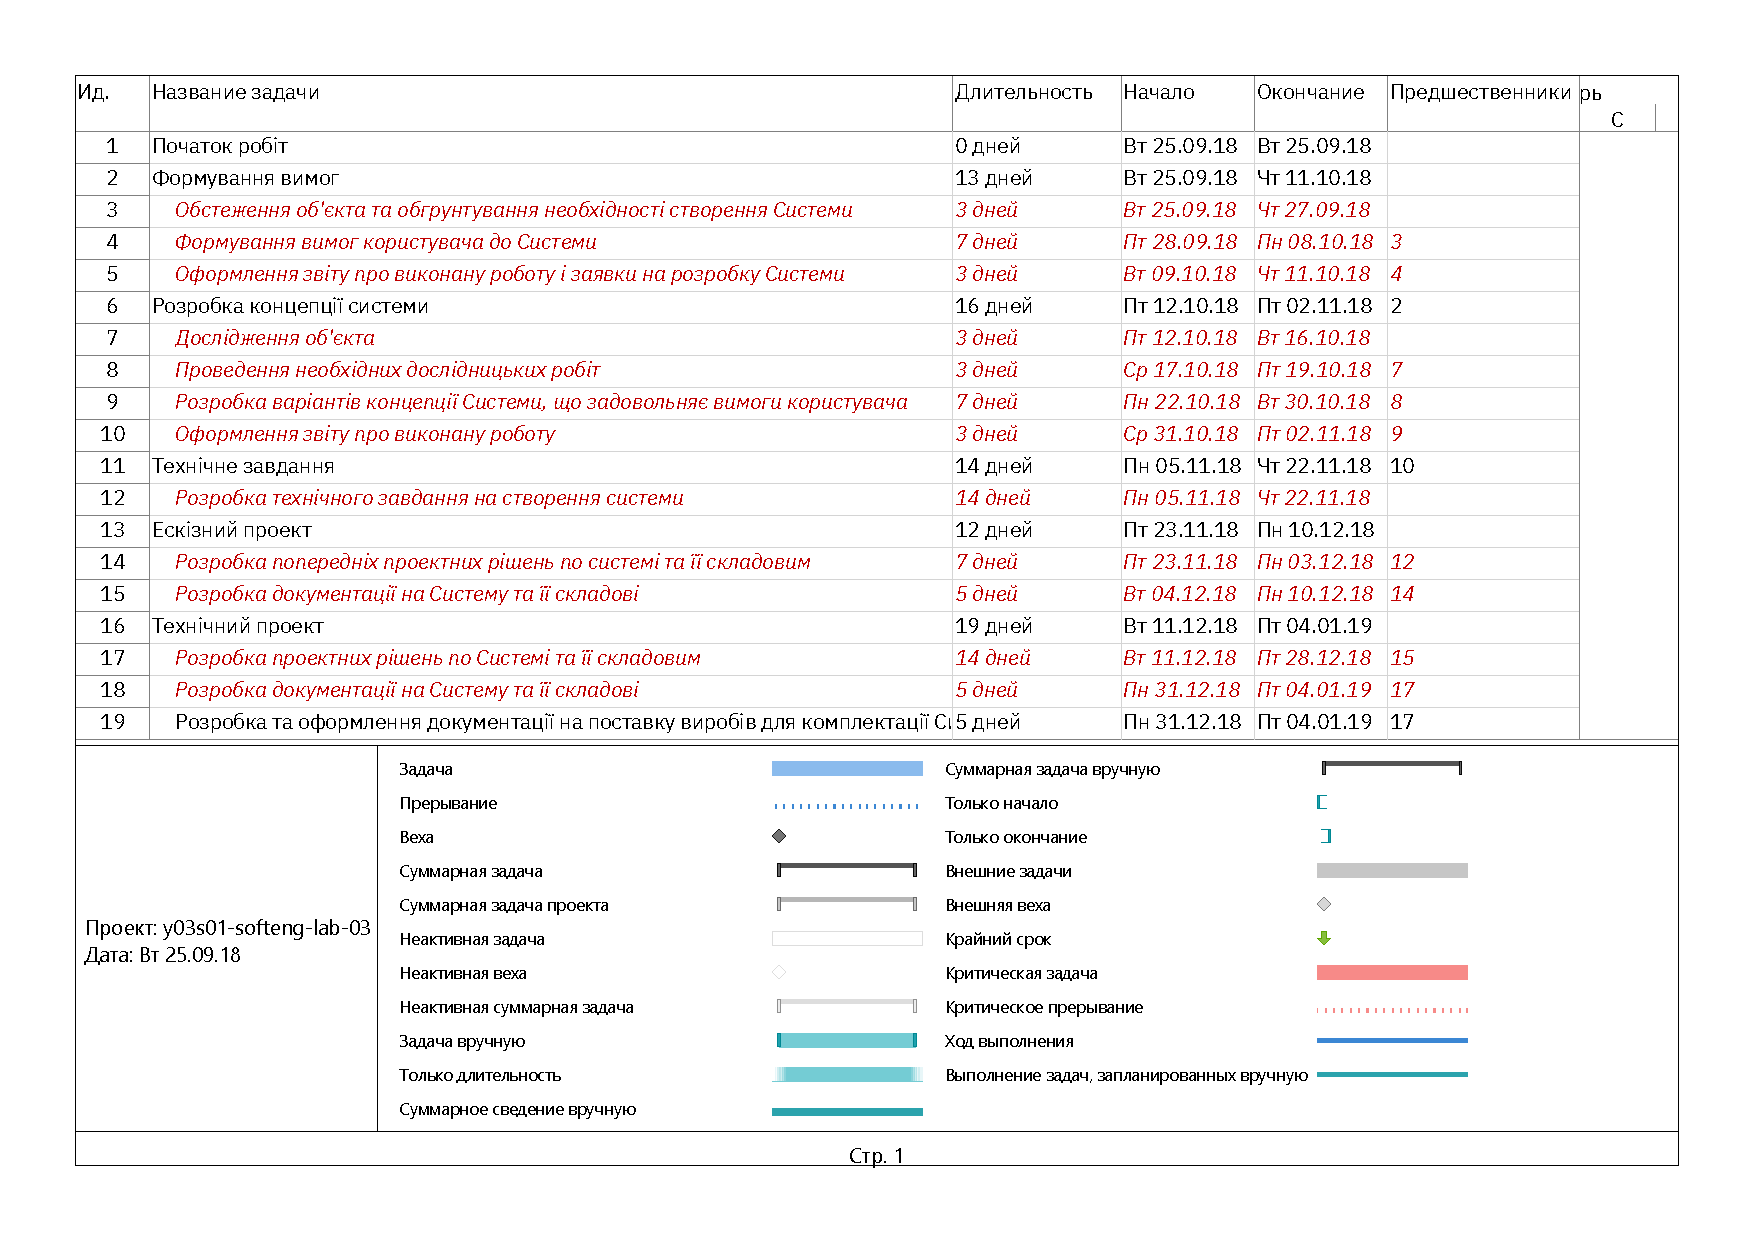
\includepdf[pages=-, landscape]{./assets/y03s01-softeng-lab-03-v02.pdf}

\end{document}
